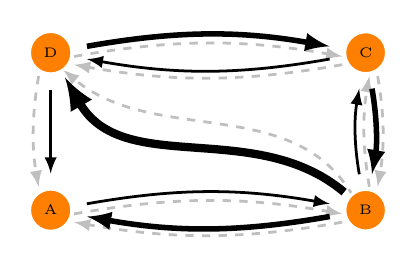
\begin{tikzpicture}[font=\tiny, >=latex, shorten >=5pt, shorten <=5pt]
    \tikzstyle{nonode} = []
    \tikzstyle{node_style} = [draw=white, very thick, circle, fill=orange]
    \tikzstyle{black_arrow1} = [->, black, line width=1]
    \tikzstyle{black_arrow2} = [->, black, line width=2]
    \tikzstyle{black_arrow3} = [->, black, line width=3]
    \tikzstyle{grey_arrow} = [->, lightgray, dashed, line width=1]

    \node[nonode] (nAd) at (0,-0.1) {};
    \node[nonode] (nAl) at (-0.1,0) {};
    \node[nonode] (nBd) at (4,-0.1) {};
    \node[nonode] (nBr) at (4.1,0) {};
    \node[nonode] (nCd) at (4,1.9) {};
    \node[nonode] (nCr) at (4.1,2) {};
    \node[nonode] (nDd) at (0,1.9) {};
    \node[nonode] (nDl) at (-0.1,2) {};

    \draw[grey_arrow] (nAd) edge [bend left=10] (nBd);
    \draw[grey_arrow] (nBd) edge [bend left=10] (nAd);
    \draw[grey_arrow] (nBr) edge [bend left=10] (nCr);
    \draw[grey_arrow] (nCr) edge [bend left=10] (nBr);
    \draw[grey_arrow] (nCd) edge [bend left=10] (nDd);
    \draw[grey_arrow] (nDd) edge [bend left=10] (nCd);
    \draw[grey_arrow] (nDl) edge [bend right=10] (nAl);
    \draw[grey_arrow] (nBd) edge [out=120, in=-40] (nDl);

    \node[node_style] (nA) at (0,0) {A};
    \node[node_style] (nB) at (4,0) {B};
    \node[node_style] (nC) at (4,2) {C};
    \node[node_style] (nD) at (0,2) {D};

    \draw[black_arrow1] (nA) edge [bend left=10] (nB);
    \draw[black_arrow2] (nB) edge [bend left=10] (nA);
    \draw[black_arrow1] (nB) edge [bend left=10] (nC);
    \draw[black_arrow2] (nC) edge [bend left=10] (nB);
    \draw[black_arrow1] (nC) edge [bend left=10] (nD);
    \draw[black_arrow2] (nD) edge [bend left=10] (nC);
    \draw[black_arrow1] (nD) edge (nA);

    \draw[black_arrow3, shorten <=2pt, shorten >=2pt] (nB) edge [out=140, in=-60] (nD);
\end{tikzpicture}
